\documentclass [10pt]{article}
\textheight	8.7in
\textwidth	6.5in
\topmargin	    0in
\oddsidemargin  0in
\evensidemargin 0in
\baselineskip 15pt

\usepackage{amssymb,amsmath,amstext}
\usepackage{amsfonts}
\usepackage{mathtools}
\usepackage{tikz}
\usetikzlibrary{automata,arrows,calc,positioning}

\begin{document}
\title{Theory of Computation Assignment no. 7}
\author{Goktug Saatcioglu}
\date{}
\maketitle
\begin{enumerate}
	\item[\textbf{(1)}]
	\begin{enumerate}
		\item[a.]This CFG describes the language of balanced (legal) parantheses. That is, each opening bracket "(" has a corresponding closing bracket ")". Notice that the empty string, $\lambda$, is not a part of this language thus the language requires at least a single pair of balanced paranthesis.
		\item[b.]Assuming that each "(" must have a corresponding ")" and each "[" must have a corresponding "]", consider the following CFG $G^{\prime}$:
		\begin{align}
			S &\rightarrow SS\:|\:(S)\:|\:[S]\:|\:()\:|\:[] \nonumber
		\end{align}
		which derives the language described in the question.
	\end{enumerate}
	\item[\textbf{(2)}]
	\begin{enumerate}
		\item[i.]To build this PDA we first construct three different PDA's based on the different cases that can occur in $A$ and take the union of them. The first case is if $\left|u\right|-\left|v\right| < 0$, then we should only accept words that are $\left|x\right|-\left|y\right| < 0$ and $\left|u\right|-\left|v\right| = \left|x\right|-\left|y\right|$. The PDA that recognize this case, say $A_{1}$, is given below.\\
		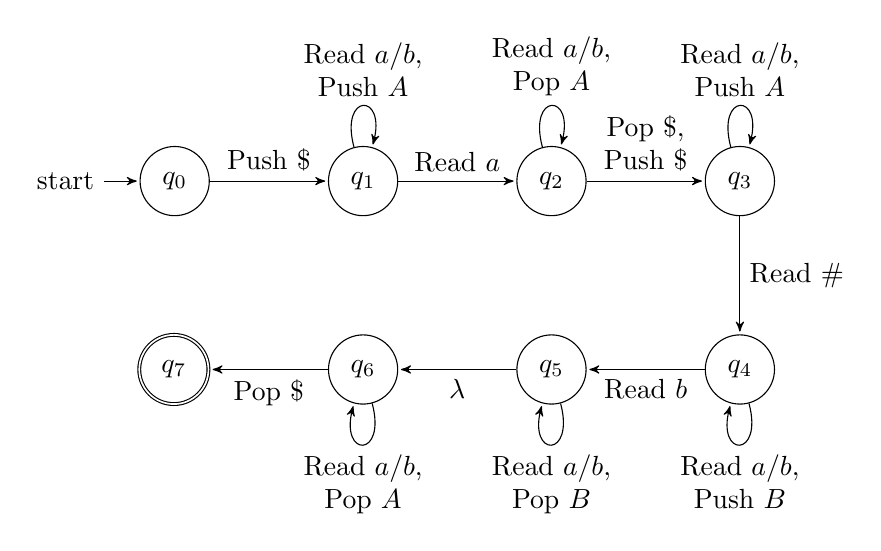
\begin{tikzpicture}[baseline=(q_0.north),>=stealth',shorten >=1pt, auto,node distance=1.5cm,align=center]
			\node[state,initial] (q_0) {$q_{0}$};
			\node[state] [right=of q_0] (q_1) {$q_{1}$};
			\node[state] [right=of q_1] (q_2) {$q_{2}$};
			\node[state] [right=of q_2] (q_3) {$q_{3}$};
			\node[state] [below=of q_3] (q_4) {$q_{4}$};
			\node[state] [left=of q_4] (q_5) {$q_{5}$};
			\node[state] [left=of q_5] (q_6) {$q_{6}$};
			\node[state,accepting] [left=of q_6] (q_7) {$q_{7}$};
			\path[->]
				(q_0) edge node {Push $\$$} (q_1)
				(q_1) edge [loop above] node {Read $a/b$,\\Push $A$} ()
				(q_1) edge node {Read $a$} (q_2)
				(q_2) edge [loop above] node {Read $a/b$,\\Pop $A$} ()
				(q_2) edge node {Pop $\$$,\\Push $\$$} (q_3)
				(q_3) edge [loop above] node {Read $a/b$,\\Push $A$} ()
				(q_3) edge node {Read $\#$} (q_4)
				(q_4) edge [loop below] node {Read $a/b$,\\Push $B$} ()
				(q_4) edge node {Read $b$} (q_5)
				(q_5) edge [loop below] node {Read $a/b$,\\Pop $B$} ()
				(q_5) edge node {$\lambda$} (q_6)
				(q_6) edge [loop below] node {Read $a/b$,\\Pop $A$} ()
				(q_6) edge node {Pop $\$$} (q_7);
		\end{tikzpicture}\\
		For $A_{1}$ we can interpret $\left|u\right|-\left|v\right| = \left|x\right|-\left|y\right|$ as $\left|u\right|-\left|v\right| - \left|x\right|+\left|y\right| = 0$ and since we know that $\left|u\right|-\left|v\right| < 0$ we will have to push to stack the extra $v$'s as we can't have a negative stack size. Thus, $q_{0}$ is the empty stack with nothing being read yet, $q_{1}$ is the stack with the shielding symbol and we push $A$'s as we read $u$. Then we transition to $q_{2}$ after reading the seperating letter of $u$ and $v$, which in this case is $a$, and we pop from the stack $A$'s as we read $v$. Since we have more letters in $v$ than in $u$, after we reach the $\$$ symbol in the stack at $q_{2}$ we transition to $q_{3}$. At $q_{3}$ we push the "excess" $A$'s onto the stack and upon reaching the $\#$ symbol move to $q_{4}$. Using a similar logic as we used to process $uav$, we first push $B$'s onto the stack in state $q_{4}$ as we read $x$. Then we read the sepearting letter of $x$ and $y$, which in this case is $b$, and we move to $q_{5}$. As we read letters from $y$ we pop $B$'s from the stack until we reach an $A$. Then we start popping the remaining $A$'s in state $q_{6}$. If we can pop the remaining $A$'s we know that $\left|u\right|-\left|v\right| - \left|x\right|+\left|y\right| = 0$ for the case $\left|u\right|-\left|v\right| < 0$ and $\left|x\right|-\left|y\right| < 0$. Thus, we finally pop the shielding symbol $\$$ and get to $q_{7}$ which is our accepting state.\\
		Next we consider the simpler case which is $\left|u\right|-\left|v\right| = 0$ and $\left|x\right|-\left|y\right| = 0$. The PDA that recognize this case, say $A_{2}$, is given below.\\
		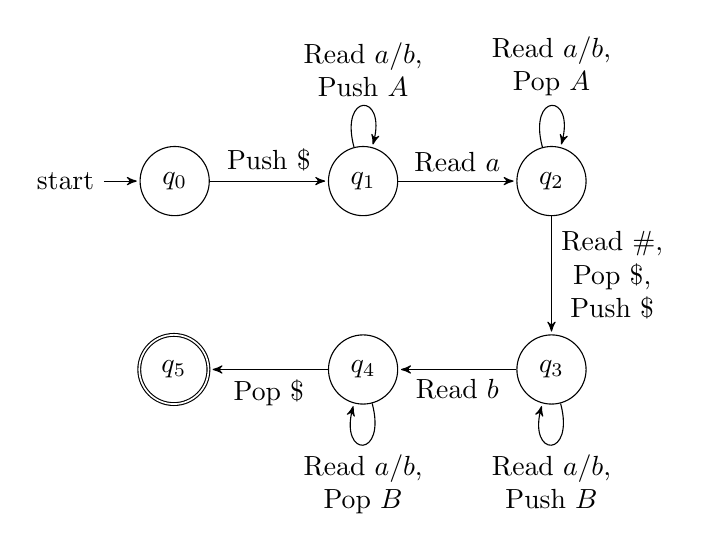
\begin{tikzpicture}[baseline=(q_0.north),>=stealth',shorten >=1pt, auto,node distance=1.5cm,align=center]
			\node[state,initial] (q_0) {$q_{0}$};
			\node[state] [right=of q_0] (q_1) {$q_{1}$};
			\node[state] [right=of q_1] (q_2) {$q_{2}$};
			\node[state] [below=of q_2] (q_3) {$q_{3}$};
			\node[state] [left=of q_3] (q_4) {$q_{4}$};
			\node[state,accepting] [left=of q_4] (q_5) {$q_{5}$};
			\path[->]
				(q_0) edge node {Push $\$$} (q_1)
				(q_1) edge [loop above] node {Read $a/b$,\\Push $A$} ()
				(q_1) edge node {Read $a$} (q_2)
				(q_2) edge [loop above] node {Read $a/b$,\\Pop $A$} ()
				(q_2) edge node {Read $\#$,\\Pop $\$$,\\Push $\$$} (q_3)
				(q_3) edge [loop below] node {Read $a/b$,\\Push $B$} ()
				(q_3) edge node {Read $b$} (q_4)
				(q_4) edge [loop below] node {Read $a/b$,\\Pop $B$} ()
				(q_4) edge node {Pop $\$$} (q_5);
		\end{tikzpicture}\\
		For $A_{2}$ the states are same as $A_{1}$ except we remove the states that count extra letters as $\left|u\right|-\left|v\right| = 0$ and $\left|x\right|-\left|y\right| = 0$. We start at state $q_{0}$ which is the empty stack and nothing has been read and at $q_{1}$ we push the shielding symbol and start counting the letters of $u$ by pushing $A$'s. After reading the seperating letter of $a$, we count the letters of $v$ by popping $A$'s in state $q_{2}$. We know this case only happens when $\left|u\right|-\left|v\right| = 0$, thus when we see $\#$ we make sure we can pop $\$$ before moving to $q_{3}$ and then push $\$$ back on the stack. Similarly, for $q_{3}$ and $q_{4}$ we count the letters of $x$ and $y$ and respectively and if $\left|x\right|-\left|y\right| = 0$ we can transition into the accepting state $q_{5}$ by popping $\$$.\\
		Finally we consider the case whhere is $\left|u\right|-\left|v\right| > 0$ and $\left|x\right|-\left|y\right| > 0$. The PDA that recognize this case, say $A_{3}$, is given below.\\
		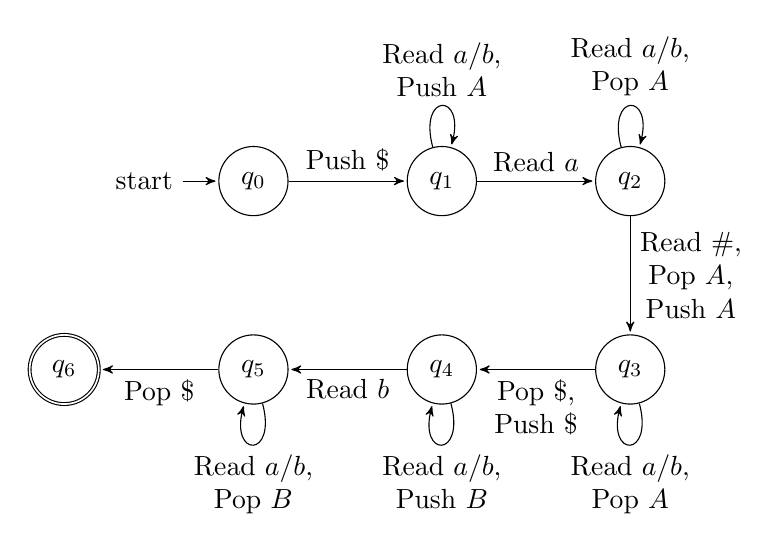
\begin{tikzpicture}[baseline=(q_0.north),>=stealth',shorten >=1pt, auto,node distance=1.5cm,align=center]
			\node[state,initial] (q_0) {$q_{0}$};
			\node[state] [right=of q_0] (q_1) {$q_{1}$};
			\node[state] [right=of q_1] (q_2) {$q_{2}$};
			\node[state] [below=of q_2] (q_3) {$q_{3}$};
			\node[state] [left=of q_3] (q_4) {$q_{4}$};
			\node[state] [left=of q_4] (q_5) {$q_{5}$};
			\node[state,accepting] [left=of q_5] (q_6) {$q_{6}$};
			\path[->]
				(q_0) edge node {Push $\$$} (q_1)
				(q_1) edge [loop above] node {Read $a/b$,\\Push $A$} ()
				(q_1) edge node {Read $a$} (q_2)
				(q_2) edge [loop above] node {Read $a/b$,\\Pop $A$} ()
				(q_2) edge node {Read $\#$,\\Pop $A$,\\Push $A$} (q_3)
				(q_3) edge [loop below] node {Read $a/b$,\\Pop $A$} ()
				(q_3) edge node {Pop $\$$,\\Push $\$$} (q_4)
				(q_4) edge [loop below] node {Read $a/b$,\\Push $B$} ()
				(q_4) edge node {Read $b$} (q_5)
				(q_5) edge [loop below] node {Read $a/b$,\\Pop $B$} ()
				(q_5) edge node {Pop $\$$} (q_6);
		\end{tikzpicture}\\
		For $A_{3}$ again we have a similar construction thus there is no need to explain all the states. However, notice that the transition from $q_{2}$ to $q_{3}$ guarantees that we only consider the case where $\left|u\right|-\left|v\right| > 0$ as we pop an $A$ and then push that $A$ back. Then we empty the stack of $A$'s as we read $x$ for state $q_{3}$. Finally, $q_{4}$ and $q_{5}$ checks if the remaining $x$ and all of $y$ have the same amount of letters and if so we move to the accepting state $q_{6}$.\\
		We can combine $A_{1}$, $A_{2}$ and $A_{3}$ by taking the union of each PDA to get a PDA, say $A_{P}$ that recognizes the language $A$. The PDA $A_{P}$ is given below.\\
		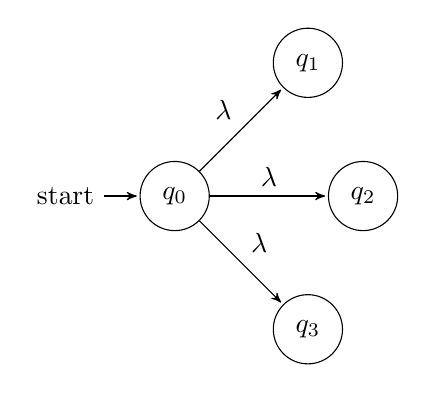
\begin{tikzpicture}[baseline=(q_0.north),>=stealth',shorten >=1pt, auto,node distance=1.5cm,align=center]
			\node[state,initial] (q_0) {$q_{0}$};
			\node[state] [above right=of q_0] (q_1) {$q_{1}$};
			\node[state] [right=of q_0] (q_2) {$q_{2}$};
			\node[state] [below right=of q_0] (q_3) {$q_{3}$};
			\path[->]
				(q_0) edge node {$\lambda$} (q_1)
				(q_0) edge node {$\lambda$} (q_2)
				(q_0) edge node {$\lambda$} (q_3);
		\end{tikzpicture}\\
		Here $q_1$ is $A_{1}$ where the $\lambda$-tranisiton goes to the starting state of $A_{1}$ and the starting state of $A_{1}$ is no longer a starting state. Similarly, $q_2$ is $A_{2}$ where the $\lambda$-tranisiton goes to the starting state of $A_{2}$ and the starting state of $A_{2}$ is no longer a starting state and $q_3$ is $A_{3}$ where the $\lambda$-tranisiton goes to the starting state of $A_{3}$ and the starting state of $A_{3}$ is no longer a starting state. We keep the accepting states of $A_{1}$, $A_{2}$ and $A_{3}$. Since $A_{P}$ covers all cases of $A$, we can say that $A_{P}$ is a PDA that recognizes $A$.
		\item[ii.]Using a similar logic to what we did for i. we can consider two possible cases. The first is when $\left|w\right| > \left|z\right|$ and the PDA that recognizes this case, say $B_{1}$, is given below.\\
		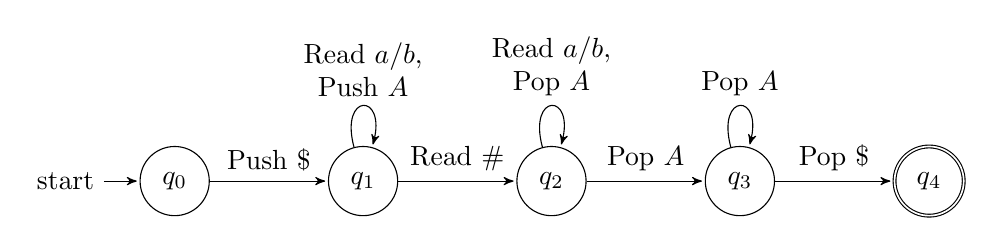
\begin{tikzpicture}[baseline=(q_0.north),>=stealth',shorten >=1pt, auto,node distance=1.5cm,align=center]
			\node[state,initial] (q_0) {$q_{0}$};
			\node[state] [right=of q_0] (q_1) {$q_{1}$};
			\node[state] [right=of q_1] (q_2) {$q_{2}$};
			\node[state] [right=of q_2] (q_3) {$q_{3}$};
			\node[state,accepting] [right=of q_3] (q_4) {$q_{4}$};
			\path[->]
				(q_0) edge node {Push $\$$} (q_1)
				(q_1) edge [loop above] node {Read $a/b$,\\Push $A$} ()
				(q_1) edge node {Read $\#$} (q_2)
				(q_2) edge [loop above] node {Read $a/b$,\\Pop $A$} ()
				(q_2) edge node {Pop $A$} (q_3)
				(q_3) edge [loop above] node {Pop $A$} ()
				(q_3) edge node {Pop $\$$} (q_4);
		\end{tikzpicture}\\
		For $B_{1}$ $q_{0}$ is the state with empty stack and nothing has been read. We push the shielding symbol $\$$ onto the stack and move to $q_{1}$ where we start counting the number of letters of $w$ by pushing $A$'s onto the stack. After seeing the $\#$ letter we move to onto $q_{2}$ where we start popping $A$'s from the stack for each letter of $z$. If there is at least one $A$ left in the stack after reading all of $z$ we know that $\left|w\right| > \left|z\right|$ and we can move to $q_{3}$. Here $q_{3}$ is necessary since there may be more $A$'s left on the stack which we'd like to empty before popping the $\$$ and moving to the accepting state $q_{4}$.\\
		Similarly, we consider the case when $\left|w\right| < \left|z\right|$ and the PDA that recognizes this case, say $B_{2}$, is given below.\\
		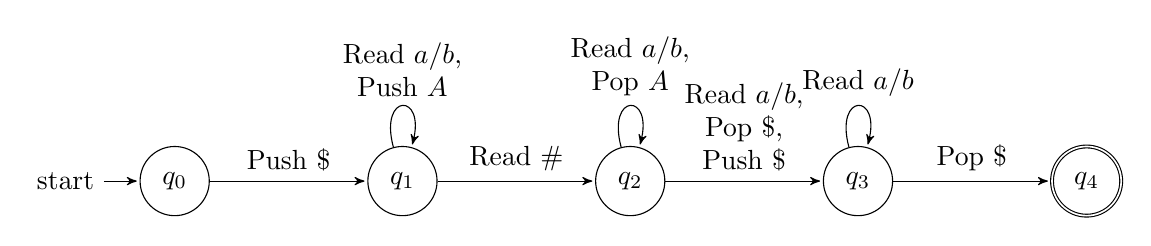
\begin{tikzpicture}[baseline=(q_0.north),>=stealth',shorten >=1pt, auto,node distance=2cm,align=center]
			\node[state,initial] (q_0) {$q_{0}$};
			\node[state] [right=of q_0] (q_1) {$q_{1}$};
			\node[state] [right=of q_1] (q_2) {$q_{2}$};
			\node[state] [right=of q_2] (q_3) {$q_{3}$};
			\node[state,accepting] [right=of q_3] (q_4) {$q_{4}$};
			\path[->]
				(q_0) edge node {Push $\$$} (q_1)
				(q_1) edge [loop above] node {Read $a/b$,\\Push $A$} ()
				(q_1) edge node {Read $\#$} (q_2)
				(q_2) edge [loop above] node {Read $a/b$,\\Pop $A$} ()
				(q_2) edge node {Read $a/b$,\\Pop $\$$,\\Push $\$$} (q_3)
				(q_3) edge [loop above] node {Read $a/b$} ()
				(q_3) edge node {Pop $\$$} (q_4);
		\end{tikzpicture}\\
		For $B_{2}$ $q_{0}$ is the state with empty stack and nothing has been read. We push the shielding symbol $\$$ onto the stack and move to $q_{1}$ where we start counting the number of letters of $w$ by pushing $A$'s onto the stack. After seeing the $\#$ letter we move to onto $q_{2}$ where we start popping $A$'s from the stack for each letter of $z$. If at one point while reading $z$ we get to the shielding symbol $\$$ and we can read at least one more letter in $z$ we know that $\left|w\right| < \left|z\right|$ and we can move to $q_{3}$. Here $q_{3}$ is necessary since there may be more letters left to read for $z$ and we'd like to read all of them before popping $\$$ and moving to the accepting state $q_{4}$.\\
		We can combine $B_{1}$, and $B_{3}$ by taking the union of each PDA to get a PDA, say $B_{P}$ that recognizes the language $B$. The PDA $B_{P}$ is given below.\\
		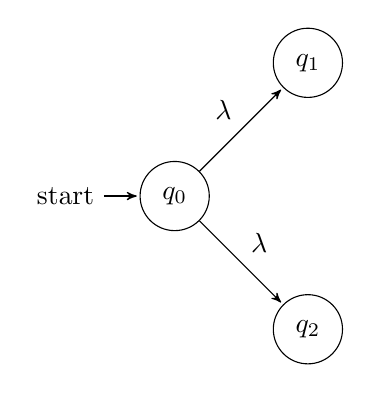
\begin{tikzpicture}[baseline=(q_0.north),>=stealth',shorten >=1pt, auto,node distance=1.5cm,align=center]
			\node[state,initial] (q_0) {$q_{0}$};
			\node[state] [above right=of q_0] (q_1) {$q_{1}$};
			\node[state] [below right=of q_0] (q_2) {$q_{2}$};
			\path[->]
				(q_0) edge node {$\lambda$} (q_1)
				(q_0) edge node {$\lambda$} (q_2);
		\end{tikzpicture}\\
		Here $q_1$ is $B_{1}$ where the $\lambda$-tranisiton goes to the starting state of $B_{1}$ and the starting state of $B_{1}$ is no longer a starting state. Similarly, $q_2$ is $B_{2}$ where the $\lambda$-tranisiton goes to the starting state of $B_{2}$ and the starting state of $B_{2}$ is no longer a starting state. We keep the accepting states of $B_{1}$ and $B_{2}$. Since $B_{P}$ covers all cases of $B$, we can say that $B_{P}$ is a PDA that recognizes $B$.
		\item[iii.]We can show that $A\cup A^{\prime}\cup B = C$ where $A^{\prime}$ is the language defined in the same way as $A$ except the letters $a$ and $b$ are switched and $C = \{s\#t\:|\:s,t\in\{a,b\}^{*} \text{ and } s\ne t\}$ by considering the cases where a word is in $C$. We know that $s \ne t$ if $\left|s\right| \ne \left|t\right|$. This is simply the language given by $B$ (would also work for the languages given by $A$ and $A^{\prime}$) and is recognized by the PDA $B_{P}$ as shown in part ii. Now it may be also true that $\left|s\right| = \left|t\right|$ but $s \ne t$. Here it is enough to show that $s$ and $t$ differ by one letter. We split this into two further cases with the first being that $s$ has an $a$ somewhere where $t$ has a $b$ in that place. This is the language $A$ since if $(\left|u\right| - \left|v\right|) = (\left|x\right| - \left|y\right|)$ then $(\left|u\right| - \left|v\right|) + \left|a\right| = (\left|x\right| - \left|y\right|) + \left|b\right|$ and we are guaranteed that $s$ and $t$ differ in a single position when $\left|s\right| = \left|t\right|$ by splitting $s$ into $uav$ and $t$ into $xby$. A is recognized by the PDA $A_{P}$ as shown in part i. Without loss of generality, we can also consider the converse case where $s$ is $ubv$ and $t$ is $xay$ such that $\left|s\right| = \left|t\right|$ but $s \ne t$. This is the language given by $A^{\prime}$ and a relevant PDA $A_{P^{\prime}}$ can be constructed by making minor modifications to $A_{P}$. Thus, we have shown that $A\cup A^{\prime}\cup B = C$ and a PDA can be constructed to recognize the language given by $C$ by simply taking the union of PDA's that recognize $A$, $A^{\prime}$ and $B$.
	\end{enumerate}
	\item[\textbf{(3)}]We begin by noting that regular expressions are made up from three base cases $\phi$ (the empty set), $\lambda$ (the languge containing the empty string) and $a$ (the language containing $a$). There are also three recursive cases where $r$ and $s$ represent languages $R$ and $S$ respectively and we have $r \cup s$ ($R \cup S$), $r \circ s$ ($R \circ S$) and $r^{*}$ ($R^{*}$). Thus, to construct a CFG that transofmrs a regular expression $w$ to a CFG $G$ such that $L(G) = L(w)$, we must handle each recursive case of regular expression. We start off by defining the rule for $a \cup b$, where $a$ and $b$ represent the languages $A$ and $B$ respectively. The corresponding CFG in this case becomes $S \rightarrow a$ and $S \rightarrow b$ because the union means $A$ or $B$ thus we can either choose the rule leading to $a$ or the rule leading to $b$. This can be simplified to just $S \rightarrow a\:|\:b$. Then we define the rule for $a \circ b$ where $a$ and $b$ represent the languages $A$ and $B$ respectively. The corresponding CFG in this case becomes $S \rightarrow ab$ since we wish to concatenate two languages $A$ and $B$ meaning we should concatenate them in the CFG. Finally, for $a^{*}$ where $a$ represents the language $A$ we will need to define the CFG rule as $S \rightarrow \lambda$ and $S \rightarrow aS$ because we can either obtain the empty string $\lambda$ for $a^{*}$ or we can derive $a$, $aa$, $aaa$... and so on for $a^{*}$. This can be simplified to just $S \rightarrow aS | \lambda$. For the base cases of regular expressions it is obvious that $\phi$ becomes $S \rightarrow S$ (i.e. the empty set), $\lambda$ becomes $S \rightarrow \lambda$ and $a$ (the single letter) becomes $S \rightarrow a$.\\Now that we have estabilished all the rules we must combine them together into an algorithm that will translate a regular expression $w$ to a CFG $G$ such that $L(G) = L(w)$. The algorithm will start reading the regular expression from the left (i.e. the beginning) and continue until it encounters one of the recursive cases described above. If a base case is encountered then the algorithm will correctly translate the regular expression to a CFG. However, if a recursive case is seen then we must act according to each case. If the union operator is seen then we recursively run the algorithm on the left of the union and on the right of the union and define a rule for the left and right as described above. Similarly, for concatention we do the same but instead of using the union rule we use the concatenation rule. For the star operator we apply its rule and apply the algorithm recursively to the expression contained in the star. Thus, as we sweep to the left we make recursive calls on each recursive operation and apply the same left sweeping algorithm to the recursive cases. Furthermore, we must stop sweeping as soon as we make a recursive call to avoid having duplicate rules which will in turn represent a different regular expression. Finally, when no recursive calls can be made we terminate using the base cases and after all calls are finished we will have converted the regular expression into a CFG. As a note, a unique naming scheme may also be used for each rule that goes to another rule to avoid duplicates.\\This algorithm works because it works the same way a regular expression is recursively generated by using recursive rules that are defined above and resolving all rules until termination cases are met. Furthermore, it takes care of duplication issues which in turn makes sure our translation is correct. Finally, termination of the algorithm is gauranteed by the base cases defined above.
\end{enumerate}

\end{document}